\documentclass{article}
\usepackage[utf8]{inputenc}
\usepackage[T1]{fontenc}
\usepackage[export]{adjustbox}
\usepackage{mathtools,amsthm,amssymb,icomma,upgreek,xfrac,enumerate, bbm,titlesec,lmodern,polski,derivative,geometry,multicol,titling,graphicx,url,amsmath,caption,lipsum,float,longtable,booktabs}
\usepackage[table,xcdraw]{xcolor}
\usepackage[hidelinks,breaklinks,pdfusetitle,pdfdisplaydoctitle]{hyperref}
\setlength{\droptitle}{-1cm}
\mathtoolsset{showonlyrefs,mathic}
\title{Komputerowa analiza szeregów czasowych raport 1}
\author{Natalia Klepacka, Joanna Kołaczek}
\date{21.12.2022}
\newtheoremstyle{break}
{\topsep}{\topsep}%
{\normalfont}{}%
{\bfseries}{}%
{\newline}{}%
\theoremstyle{break}
\newtheorem{zadanie}{Zadanie} 
\newtheorem*{rozwiazanie}{Rozwiązanie}

\titleformat*{\section}{\LARGE\bfseries}
\titleformat*{\subsection}{\Large\bfseries}
\titleformat*{\subsubsection}{\large\bfseries}
\titleformat*{\paragraph}{\large\bfseries}
\titleformat*{\subparagraph}{\large\bfseries}

\graphicspath{{obrazki/}}


\begin{document}
	\maketitle
	\tableofcontents
	\clearpage
\section{Opis danych}
	Niniejszy raport powstał na potrzeby realizacji laboratorium ze Statystyki Stosowanej, prowadzonych przez dr inż. Aleksandrę Grzesiek, do wykładu dr hab. inż. Krzysztofa Burneckiego. Będziemy analizować dane dotyczące długości ogonów myszołowów rdzawosternych (ang. red-tailed hawk) podane w milimetrach. Dysponujemy próbą o wielkości 577 pobraną \href{ https://vincentarelbundock.github.io/Rdatasets/datasets.html}{\textit{z tej strony}}. Na jej podstawie przedstawimy statystyki podzielone według miar położenia, rozproszenia, asymetrii oraz spłaszczenia. Na koniec pierwszego rozdziału zebrane wielkości przedstawimy w formie tabeli.  W~drugiej części raportu zwizualizjemy dane za pomocą histogramu oraz wykresu pudełkowego. Wyznaczymy ponadto dystrybuantę empiryczną analizowanej próby. Na koniec wyniki badań omówimy w~podsumowaniu. Życzymy Czytelnikowi miłej lektury.
	
\section{Analiza jednowymiarowa zmiennej zależnej oraz zmiennej niezależnej}

\begin{figure}[H]
	\begin{center}
		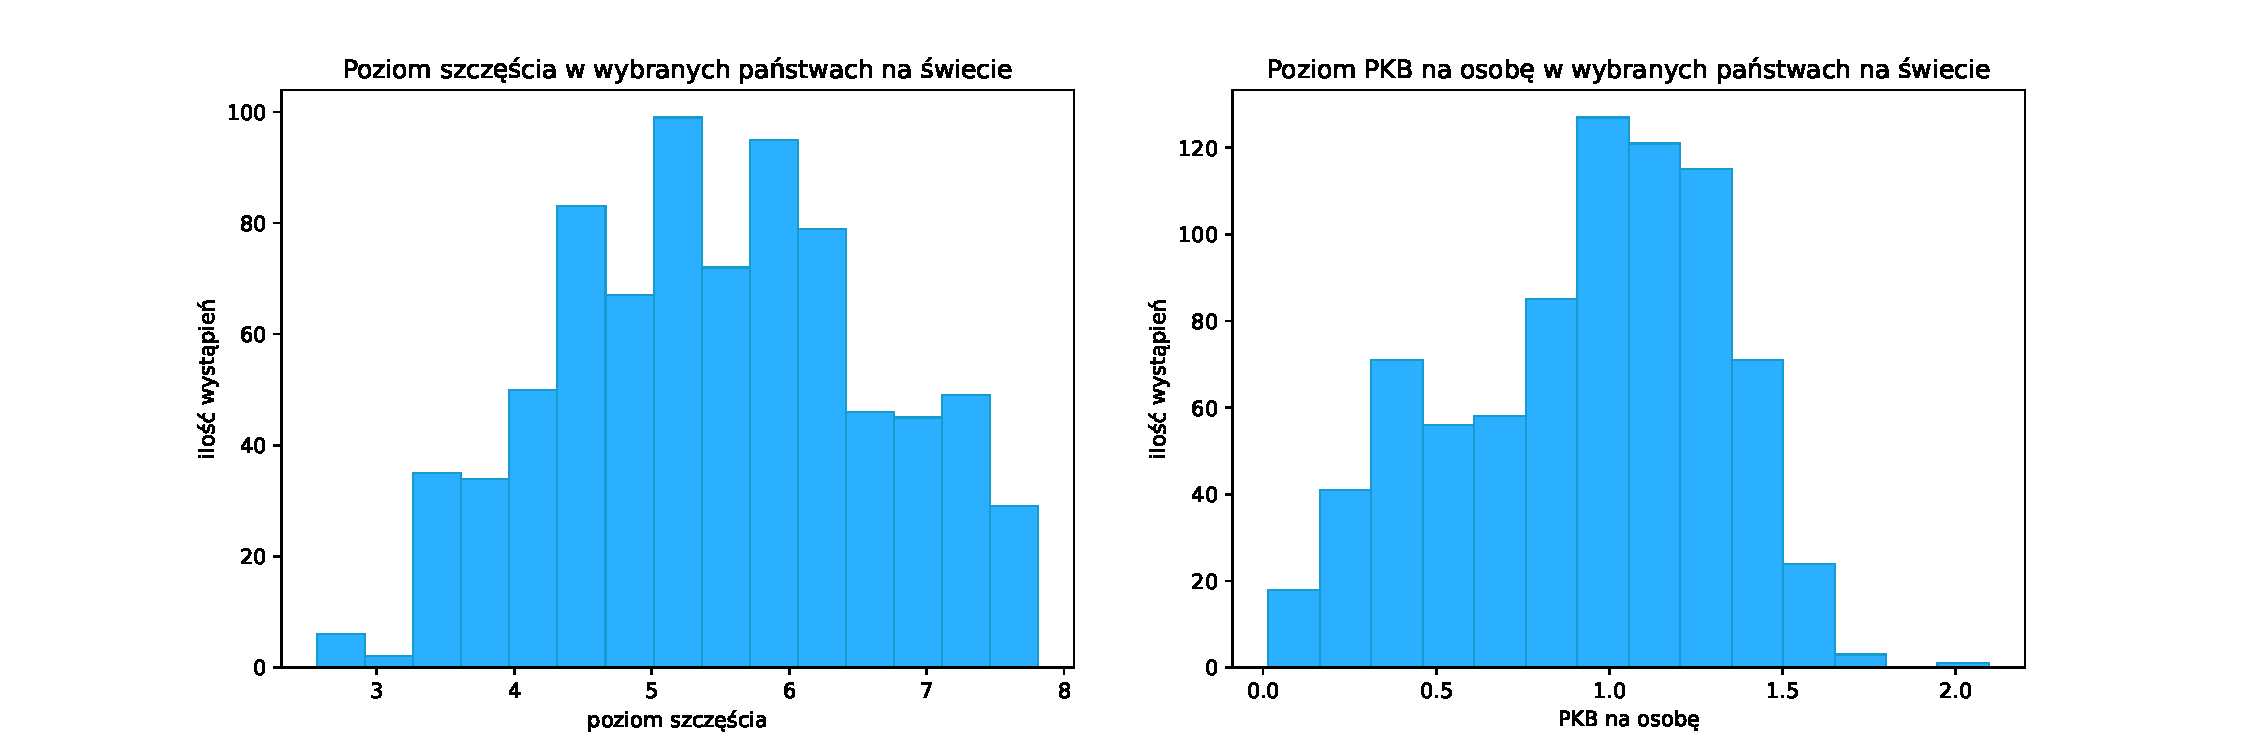
\includegraphics[scale=0.43]{hist.pdf}
		\caption{Histogramy}
		\label{fig:hist}
	\end{center}
\end{figure}

\begin{figure}[H]
	\begin{center}
		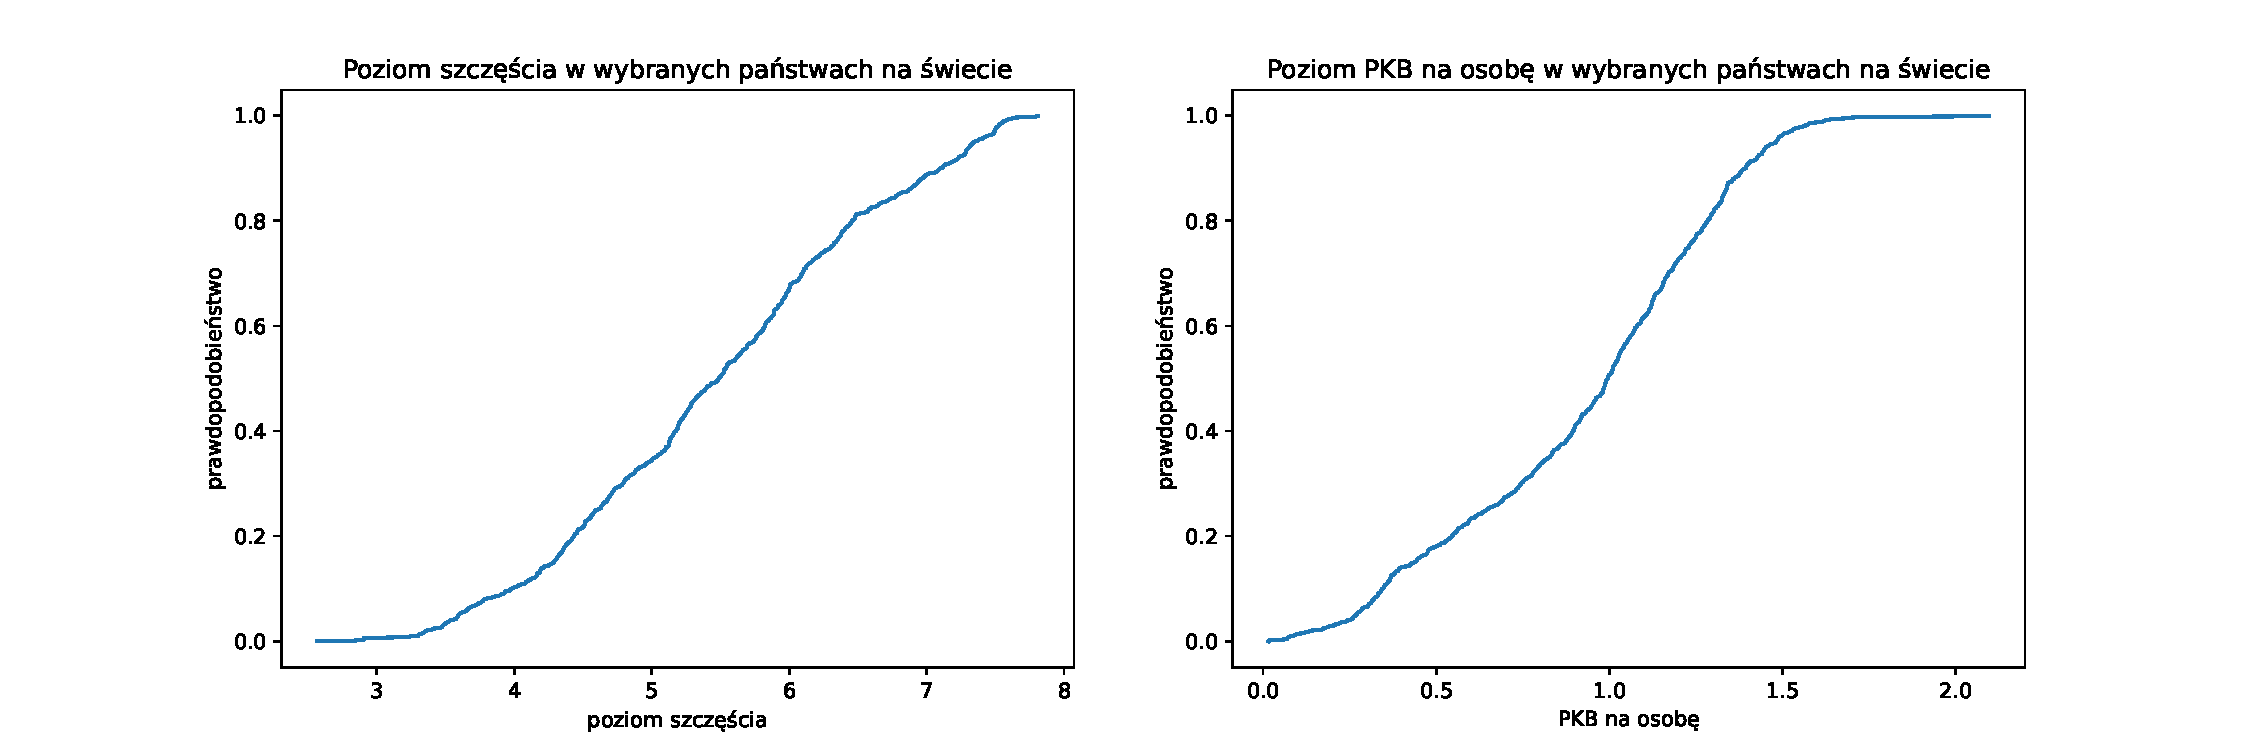
\includegraphics[scale=0.43]{distr.pdf}
		\caption{Dystrybuanta empiryczna}
		\label{fig:distr}
	\end{center}
\end{figure}

\begin{figure}[H]
	\begin{center}
		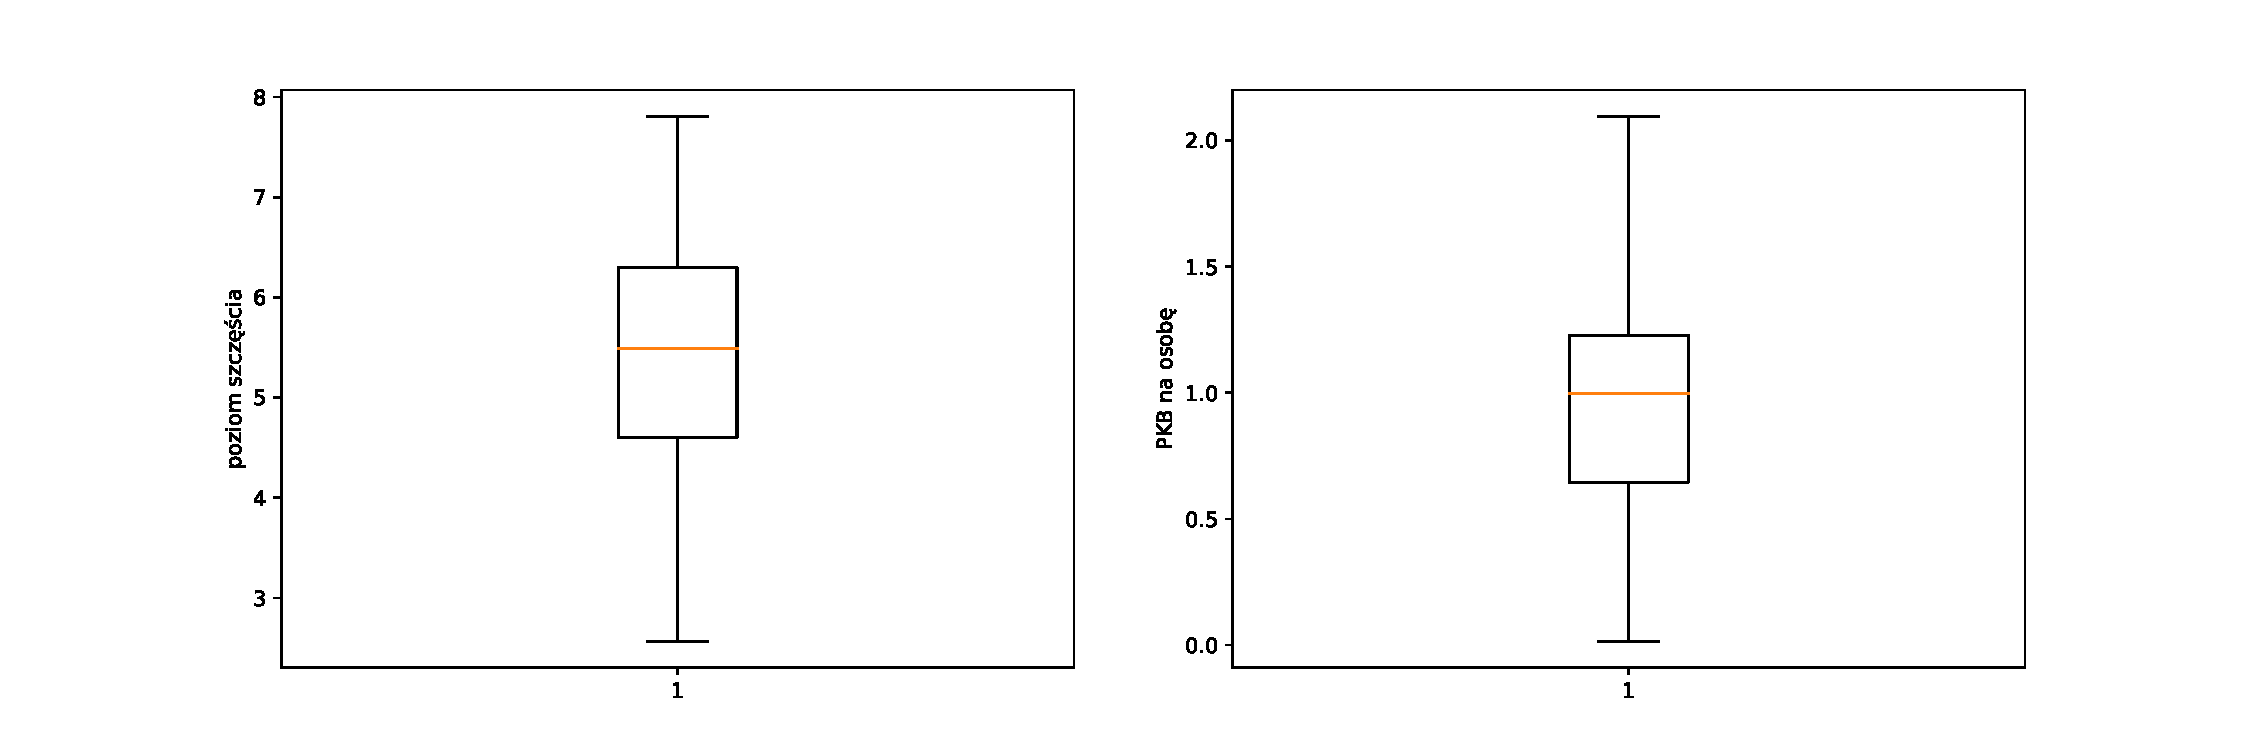
\includegraphics[scale=0.43]{box.pdf}
		\caption{Boxploty}
		\label{fig:box}
	\end{center}
\end{figure}


Na histogramie [\ref{fig:hist}] widzimy rozkład danych z badanej próby. Jest to dobry sposób wizualizacji danych, ponieważ można dzięki niemu łatwo oszacować niektóre statystyki takie jak średnia, skośność itp. Widzimy, że dla naszych danych najczęściej obserwujemy długości ogona zawarte w przedziale 220 do 225 mm.

Wykres pudełkowy (ang. \textit{boxplot}) [\ref{fig:box}] jest to graficzna reprezentacja mediany, kwartyli oraz maksimum i minimum z danych (kropki oznaczają wartości odstające), wąsy mają długość półtorej wartości rozstępu międzykwartylowego.

Dystrybuanta empiryczna [\ref{fig:dystr}] pokazuje z jakim prawdopodobieństwem natrafimy na myszołowa rdzawosternego o długości ogona mniejszej bądź równej od danej wartości. Widzimy, że szansa na to, aby spotkać osobnika z ogonem krótszym niż 200 mm lub dłuższym niż 250 mm jest nikła, natomiast długości między 200 a 250 mm występują najczęściej.

\begin{figure}[H]
	\begin{longtable}[l]{|ll|l|l|}
		\hline
		\rowcolor[HTML]{C0C0C0} 
		\multicolumn{2}{|l|}{\cellcolor[HTML]{C0C0C0}Miary}                             & Poziom szczęścia & PKB na osobe \\ \hline
		\multicolumn{1}{|l|}{}                               & średnia arytmetyczna     & 5.47             & 0.93         \\ \cline{2-4} 
		\multicolumn{1}{|l|}{}                               & średnia geometryczna     & 5.23             & 0.58         \\ \cline{2-4} 
		\multicolumn{1}{|l|}{}                               & średnia harmoniczna      & 5.35             & 0.81         \\ \cline{2-4} 
		\multicolumn{1}{|l|}{}                               & średnia ucinana 10\%     & 5.47             & 0.94         \\ \cline{2-4} 
		\multicolumn{1}{|l|}{}                               & mediana Q2               & 5.48             & 0.99         \\ \cline{2-4} 
		\multicolumn{1}{|l|}{}                               & Q1                       & 4.59             & 0.64         \\ \cline{2-4} 
		\multicolumn{1}{|l|}{położenia}    & Q3                       & 6.30             & 1.22         \\ \hline
		\multicolumn{1}{|l|}{}                               & rozstęp                  & 5.24             & 2.08         \\ \cline{2-4} 
		\multicolumn{1}{|l|}{}                               & rozstęp międzykwartylowy & 1.70             & 0.58         \\ \cline{2-4} 
		\multicolumn{1}{|l|}{}                               & wariancja nieobciążona   & 1.26             & 0.14         \\ \cline{2-4} 
		\multicolumn{1}{|l|}{}                               & odchylenie standardowe   & 1.12             & 0.38         \\ \cline{2-4} 
		\multicolumn{1}{|l|}{rozproszenia} & współczynnik zmienności  & 20.52            & 41.33        \\ \hline
		\multicolumn{1}{|l|}{spłaszczenia}                   & kurtoza                  & 2.25             & 2.31         \\ \hline
		\multicolumn{1}{|l|}{skośności}                      & skośność                 & -0.01            & -0.36        \\ \hline
	\end{longtable}
	\caption{Zestawienie omówionych statystyk}
\end{figure}
	
\section{Analiza zależności liniowej pomiędzy zmienną zależną a zmienną niezależną}

\subsection{Wykres rozproszenia i określenie zależności}

\begin{figure}[H]
	\begin{center}
		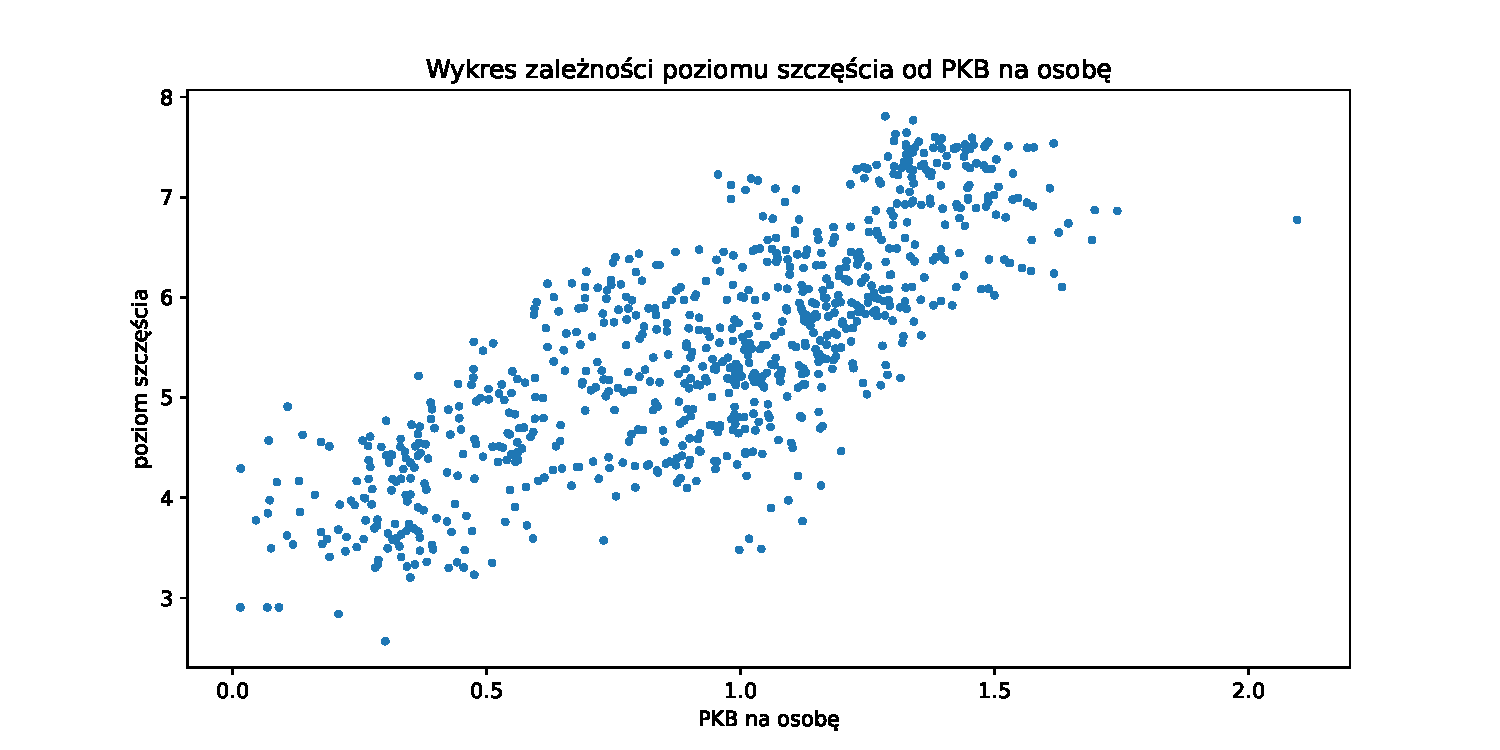
\includegraphics[scale=0.43]{plot1.pdf}
		\caption{wykres rozproszenia}
		\label{fig:rozproszenie}
	\end{center}
\end{figure}

Na podstawie wykresu rozproszenia [\ref{fig:rozproszenie}] możemy stwierdzić, że zależność pomiędzy zmiennymi prawdopodobnie jest liniowa.

\subsection{Punktowa estymacja współczynników}

Współczynniki regresji liniowej wyznaczamy ze wzorów
\begin{equation}
\left\{ \begin{array}{ll}
	\beta_{1} = r\frac{S_{y}}{S_{x}}\\
	\beta_{0} = \bar{y} - r\beta_{1}\bar{x}
\end{array} \right.,
\end{equation} gdzie
\begin{equation}
	r = \frac{1}{n-1}\frac{\sum_{i=1}^{n}(x_i-\bar{x})(y_i-\bar{y})}{S_{x}S_{y}},
\end{equation}
\begin{equation}
	S_{x} = \sqrt{\frac{1}{n-1}\sum_{i=1}^{n}(x_{i}-\bar{x})^{2}},
\end{equation}
\begin{equation}
	S_{y} = \sqrt{\frac{1}{n-1}\sum_{i=1}^{n}(y_{i}-\bar{y})^{2}},
\end{equation}
\begin{equation}
	\bar{x} = \frac{1}{n}\sum_{i=1}^{n}x_{i},
\end{equation}
\begin{equation}
	\bar{y} = \frac{1}{n}\sum_{i=1}^{n}y_{i}.
\end{equation}

Wzory te zostały wyznaczone przy pomocy metody najmniejszych kwadratów.

\begin{figure}[H]
	\begin{center}
		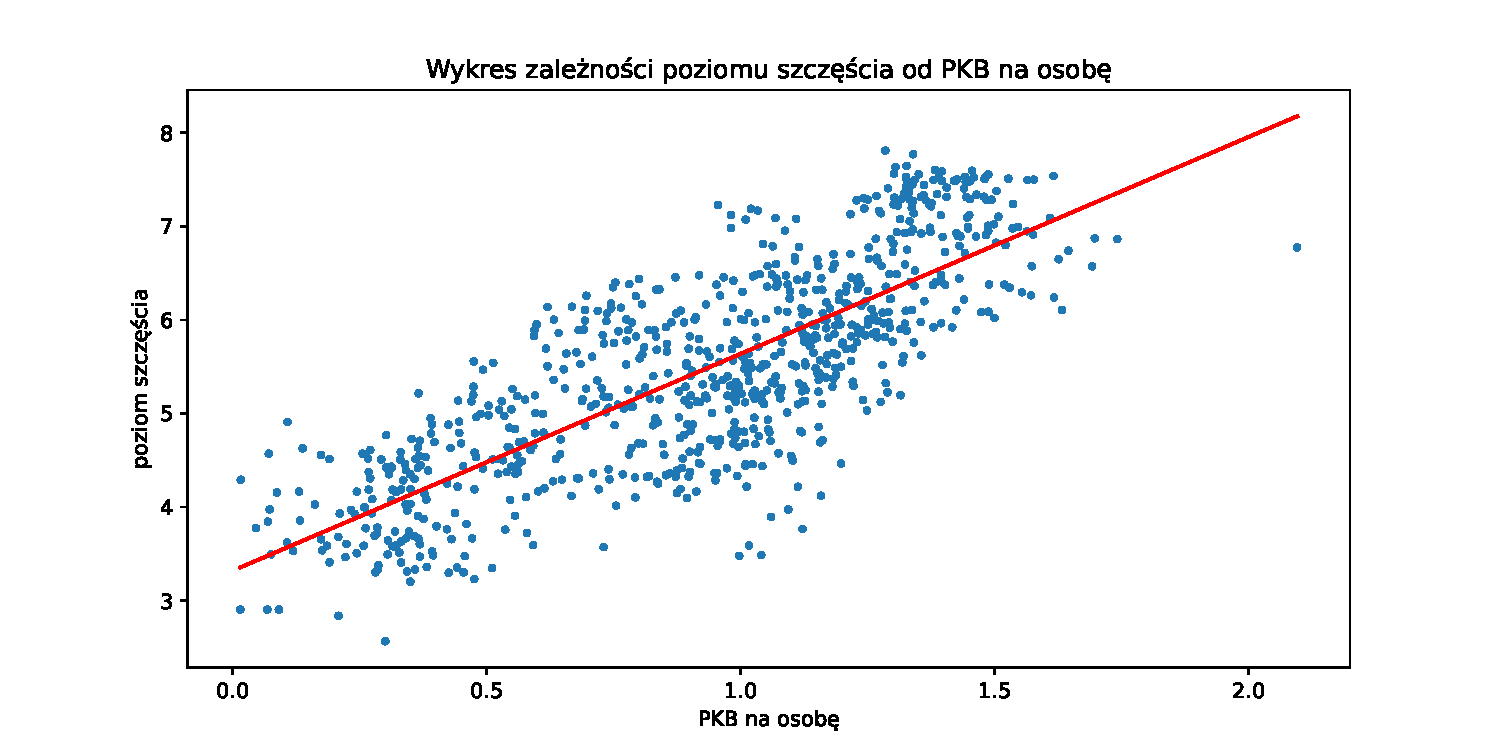
\includegraphics[scale=0.43]{plot2.pdf}
		\caption{wykres rozproszenia z zaznaczoną prostą regresji}
		\label{fig:prosta}
	\end{center}
\end{figure}

Z powyższych wzorów otrzymaliśmy 
\begin{equation}
	\left\{ \begin{array}{ll}
		\beta_{1} \approx 2.32\\
		\beta_{0} \approx 3.32
	\end{array} \right..
\end{equation}
Współczynniki te opisują prostą widoczną na wykresie [\ref{fig:prosta}].

\subsection{Przedziałowa estymacja współczynników}

Z założenia o normalności rozkładu $\{\varepsilon\}_{i=1}^{n}$, przy braku znajomości jego wariancji możemy stwierdzić, że unormowane parametry $\beta_0$, $\beta_1$ mają rozkład t-studenta z n-2 stopniami swobody. Przedziały ufności przyjmują wtedy postać
\begin{equation}
\left\{ \begin{array}{ll}
	P\left(\hat{\beta}_{0}-t_{n-2}(1-\frac{\alpha}{2})S\sqrt{\frac{1}{n}+\frac{\bar{x}^{2}}{\sum_{i=1}^{n}(x_i-\bar{x})^2}} < \beta_{0} < \hat{\beta}_{0}+t_{n-2}(1-\frac{\alpha}{2})S\sqrt{\frac{1}{n}+\frac{\bar{x}^{2}}{\sum_{i=1}^{n}(x_i-\bar{x})^2}}\right) = 1-\alpha\\
	P\left(\hat{\beta}_{1}-t_{n-2}(1-\frac{\alpha}{2})\frac{S}{\sqrt{\sum_{i=1}^{n}(x_i-\bar{x})^2}} < \beta_{1} < \hat{\beta}_{1}+t_{n-2}(1-\frac{\alpha}{2})\frac{S}{\sqrt{\sum_{i=1}^{n}(x_i-\bar{x})^2}}\right) = 1-\alpha
\end{array} \right.,
\end{equation} gdzie
\begin{equation}
	S = \sqrt{\frac{\sum_{i=1}^{n}(y_i - \hat{y}_i)^2}{n-2}}.
\end{equation}
Przyjmując $\alpha = 0.05$ otrzymujemy zatem, że z 95\% prawdopodobieństwem
\begin{equation}
	\left\{ \begin{array}{ll}
		\beta_{1} \in (2.19, 2.44)\\
		\beta_{0} \in (3.20, 3.44)
	\end{array} \right..
\end{equation}

\subsection{Ocena poziomu zależności}

\subsection{Predykcja oraz jej przedziały ufności}

\subsection{Interpretacja wyników}

\section{Analiza residuów}

\begin{figure}[H]
	\begin{center}
		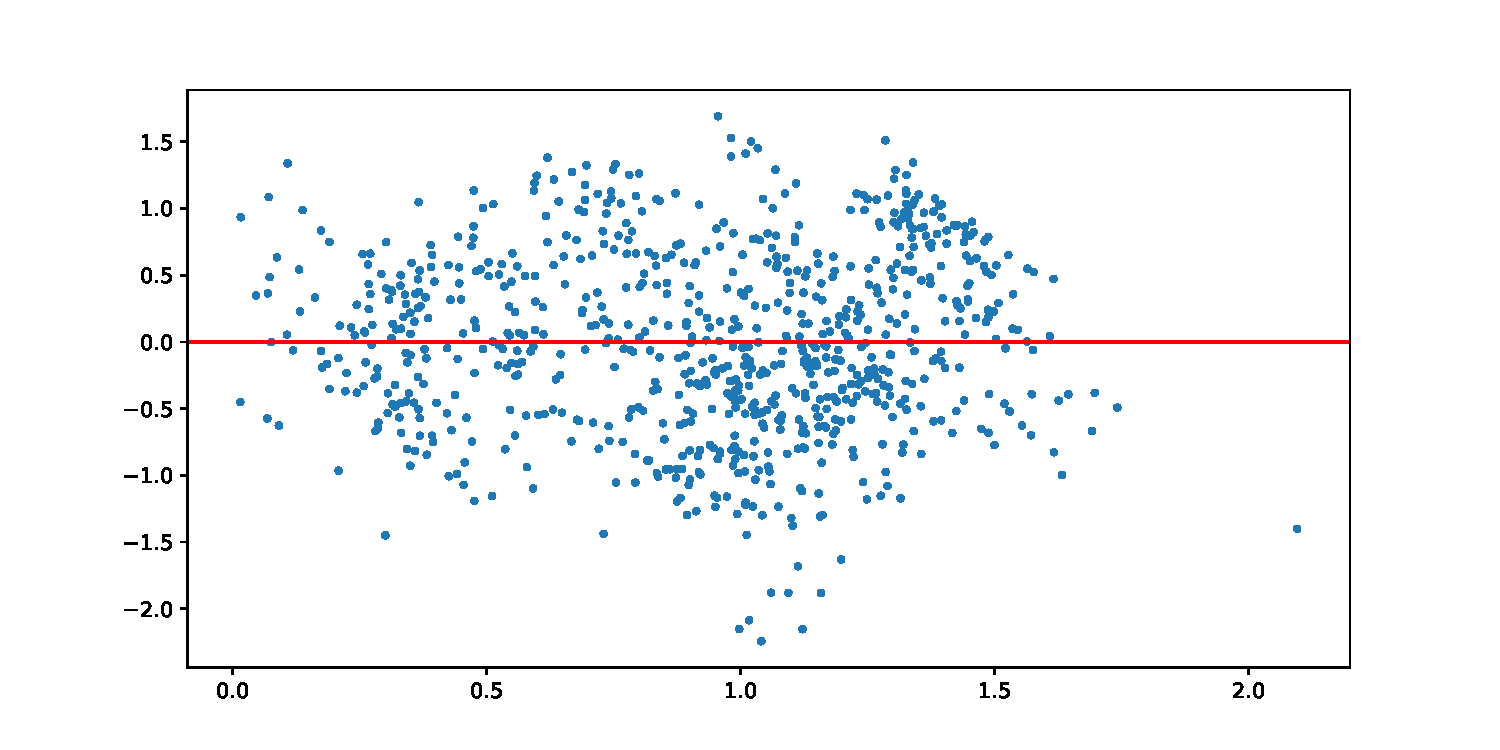
\includegraphics[scale=0.43]{res.pdf}
		\caption{Wy}
		\label{fig:res}
	\end{center}
\end{figure}

\begin{figure}[H]
	\begin{center}
		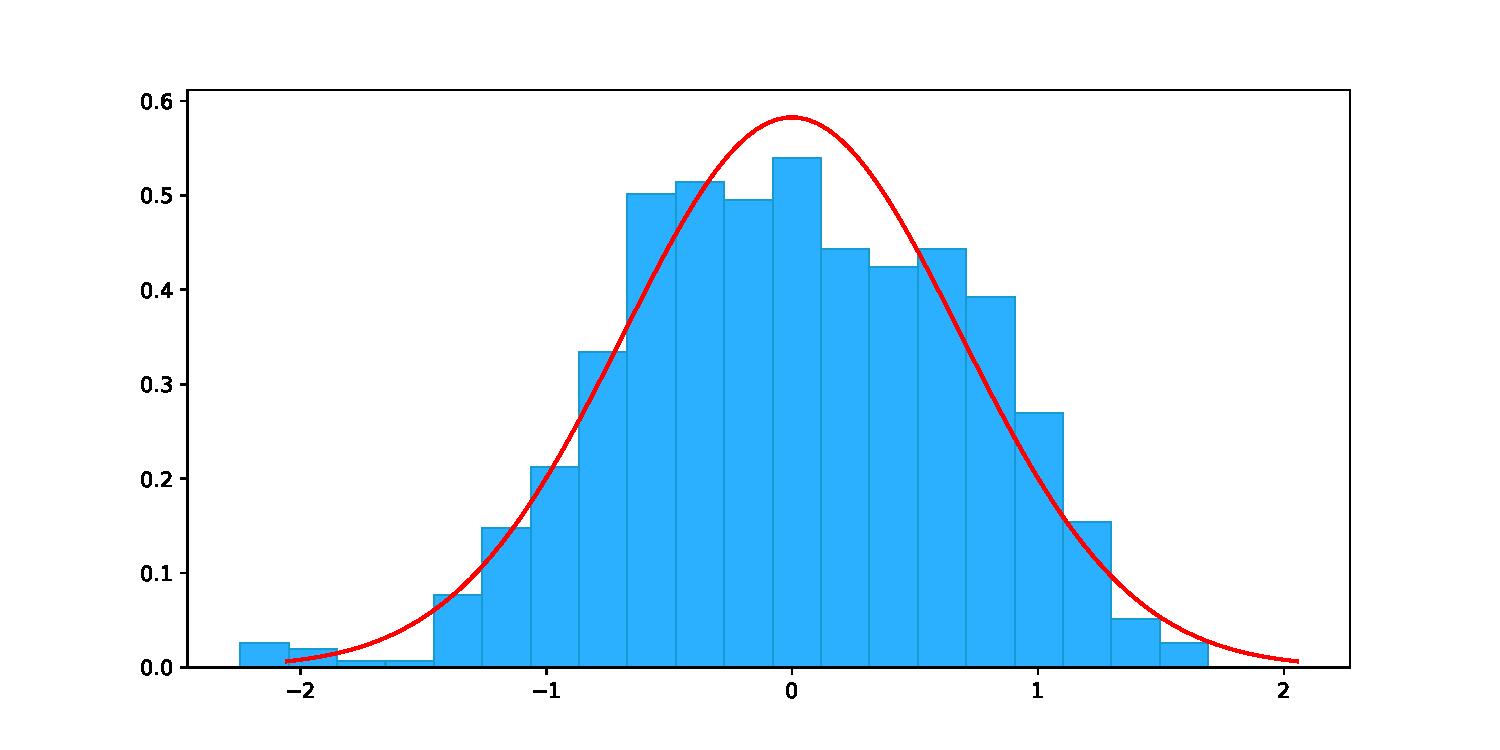
\includegraphics[scale=0.43]{res_hist.pdf}
		\caption{Wy}
		\label{fig:res_hist}
	\end{center}
\end{figure}

	
\section{Podsumowanie}
	Analizując przedstawione w raporcie statystyki możemy sformułować następujące wnioski i przypuszczenia dotyczące długości ogonów w populacji myszołowów rdzawosternych. Z histogramu widzimy, że badany rozkład przypomina rozkład normalny, jednak po obliczeniu skośności okazuje się, że różni się ona od skośności rozkładu normalnego, która wynosi zero. Podejrzewamy, iż może to być spowodowane licznością próby. Statystyczny myszołów rdzawosterny powinien mieć ogon o długości od $207,638$ do $236.66$ mm, (średnia arytmetyczna $\pm$ odchylenie standardowe). Biorąc średnią z populacji przewidujemy długość około $222,15$ mm. Wartości skrajne nie wpływają znacząco na wartość średniej - wiemy to po obliczeniu średniej Winsorowskiej ($222,182$ mm) i ucinanej ($222,104$ mm). 
	
	\section{Źródła}
	\begin{itemize}
		\item Wykłady
		\item \url{https://vincentarelbundock.github.io/Rdatasets/csv/Stat2Data/HawkTail.csv}
		\item \url{https://www.geo.fu-berlin.de/en/v/soga/Basics-of-statistics/Descriptive-Statistics/Measures-of-Position/index.html}
		\item \url{https://www.investopedia.com/terms/w/winsorized_mean.asp}
	\end{itemize}
	
	
\end{document}